\chapter{Constraint Satisfaction}
In this chapter we discuss algorithms for solving 
\href{https://en.wikipedia.org/wiki/Constraint_satisfaction_problem}{constraint satisfaction problems}.
These problems can be seen as a refinement of the search problems discussed in the previous chapter:  In a
search problem, the states are abstract and therefore have no structure that can be exploited to guide the
search.  In a \blue{constraint satisfaction problem}, the states have a structure that can be exploited to
guide the search.  This chapter is structured as follows:
\begin{enumerate}
\item The first section defines the notion of a constraint satisfaction problem.  In order to illustrate this
      concept, two examples of constraint satisfaction problems are presented.  After that, we discuss
      applications of constraint satisfaction problems.
\item The simplest algorithm to solve a constraint satisfaction problem is via \blue{brute force search}.
      The idea behind brute force search is to test all possible variable assignments.
\item In most cases, the search space is too big to be enumerated completely.
      \blue{Backtracking search} improves on brute force search by mixing the generation
      of assignments with the testing of the constraints.  In many cases, this approach can
      drastically improve the performance of the search algorithm.
\item Backtracking search can be refined by using \blue{constraint propagation} and by
      using the \blue{most restricted variable} heuristic.
\item Furthermore, checking the \blue{consistency} of the values assigned to different variables
      can reduce the size of the search space considerably. 
\item Finally, \blue{local search} is a completely different approach to solve
      constraint satisfaction problems.
\end{enumerate}

\section{Formal Definition of Constraint Satisfaction Problems}
Formally, we define a 
\href{https://en.wikipedia.org/wiki/Constraint_satisfaction_problem}{constraint satisfaction problem} as a triple
\\[0.2cm]
\hspace*{1.3cm}
$\mathcal{P} := \langle \mathtt{Vars}, \mathtt{Values}, \mathtt{Constraints} \rangle$
\\[0.2cm]
where
\begin{enumerate}
\item $\mathtt{Vars}$ is a set of strings which serve as \blue{variables},
\item $\mathtt{Values}$ is a set of \blue{values} that can be assigned to the variables in $\mathtt{Vars}$.
\item $\mathtt{Constraints}$ is a set of formul\ae\ from \blue{first order logic}.  Each of these formul\ae\ is
      called a \blue{constraint} of $\mathcal{P}$.

      In order to be able to interpret these formul\ae, we need a \blue{first order structure} $\mathcal{S} = \langle \mathcal{U}, \mathcal{J} \rangle$.  
      Here, $\mathcal{U}$ is the \blue{universe} of $\mathcal{S}$ and we will assume that this
      universe is identical to the set $\mathtt{Values}$, that is we have
      \\[0.2cm]
      \hspace*{1.3cm}
      $\mathcal{U} = \texttt{Values}$.
      \\[0.2cm]
      The second component $\mathcal{J}$ defines the
      \blue{interpretations} of the function symbols and predicate symbols that are used in the formul\ae\
      defining the constraints.  In what follows we assume that these interpretations are understood from the
      context of the constraint satisfaction problem $\mathcal{P}$.
\end{enumerate}
In the following, the abbreviation \textsc{Csp} is short for \blue{constraint satisfaction problem}.
Given a \textsc{Csp}
\\[0.2cm]
\hspace*{1.3cm}
 $\mathcal{P} = \langle \mathtt{Vars}, \mathtt{Values}, \mathtt{Constraints} \rangle$, 
\\[0.2cm]
a \blue{variable assignment} for $\mathcal{P}$ is a function
\\[0.2cm]
\hspace*{1.3cm}
$A: \mathtt{Vars} \rightarrow \mathtt{Values}$.
\\[0.2cm]
A variable assignment $A$ is a \blue{solution} of the \textsc{Csp} $\mathcal{P}$ 
if, given the assignment $A$, all constraints of $\mathcal{P}$ are satisfied.
Finally, a \blue{partial variable assignment} $B$ for $\mathcal{P}$ is a function
\\[0.2cm]
\hspace*{1.3cm}
$B: \mathtt{Vars} \rightarrow \mathtt{Values} \cup \{ \Omega \}$ \quad where $\Omega$ denotes the undefined value.
\\[0.2cm]
Hence, a partial variable assignment does not assign values to all variables.  Instead, it assigns values only
to a subset of the set $\mathtt{Vars}$.  The \blue{domain} $\mathtt{dom}(B)$ of a partial variable assignment $B$ is the
set of those variables that are assigned a value different from $\Omega$, i.e.~we define
\\[0.2cm]
\hspace*{1.3cm}
$\mathtt{dom}(B) := \bigl\{ x \in \mathtt{Vars} \mid B(x) \not= \Omega \bigr\}$.
\\[0.2cm]
We proceed to illustrate the definitions given so far with two examples.


\begin{figure}[!ht]
  \centering
  \framebox{
\epsfig{file=Figures/australia.pdf,scale=0.8}} 
  \caption{A map of Australia.}
  \label{fig:australia.pdf}
\end{figure}

\subsection{Example: Map Colouring}
In \href{https://en.wikipedia.org/wiki/Four_color_theorem}{map colouring} a map showing different state
borders is given and the task is to colour the different states such that no two states that have a common
border share the same colour.  \myFig{australia.pdf} shows a map of Australia.  There are seven different
states in Australia:
\begin{enumerate}
\item Western Australia, abbreviated as $\mathrm{WA}$,
\item Northern Territory, abbreviated as $\mathrm{NT}$,
\item South Australia, abbreviated as $\mathrm{SA}$,
\item Queensland, abbreviated as $\mathrm{Q}$,
\item New South Wales, abbreviated as $\mathrm{NSW}$,
\item Victoria, abbreviated as $\mathrm{V}$, and
\item Tasmania, abbreviated as $\mathrm{T}$.
\end{enumerate}
Figure \ref{fig:australia.pdf} would certainly look better if different states had been coloured with different
colours.  For the purpose of 
this example let us assume that we have only three colours available.  The question then is whether it is 
possible to colour the different states in a way that no two neighbouring states share the same colour.  This
problem can be formalized as a constraint satisfaction problem.  To this end we define:
\begin{enumerate}
\item $\texttt{Vars} := \{ \mathrm{WA}, \mathrm{NT}, \mathrm{SA}, \mathrm{Q}, \mathrm{NSW}, \mathrm{V}, \mathrm{T} \}$,
\item $\texttt{Values} := \{ \texttt{red}, \texttt{green}, \texttt{blue} \}$,
\item $\texttt{Constraints} := $ \\[0.1cm]
      \hspace*{0.3cm}
      $\bigl\{ \mathrm{WA} \not= \mathrm{NT}, \mathrm{WA} \not= \mathrm{SA},
                 \mathrm{NT} \not= \mathrm{SA}, \mathrm{NT} \not= \mathrm{Q},
                 \mathrm{SA} \not= \mathrm{Q},  \mathrm{SA} \not= \mathrm{NSW}, \mathrm{SA} \not= \mathrm{V}, 
                 \mathrm{Q}  \not= \mathrm{NSW},
                 \mathtt{NSW}\not= \mathtt{V}, 
                 \mathrm{V}  \not= \mathrm{T}
       \bigr\}
      $
\end{enumerate}
Then $\mathcal{P} := \langle \texttt{Vars}, \texttt{Values}, \texttt{Constraints} \rangle$ is a constraint satisfaction problem.  
If we define the assignment $A$ such that
\begin{enumerate}
\item $A(\mathrm{WA}) = \texttt{blue}$,
\item $A(\mathrm{NT}) = \texttt{red}$,
\item $A(\mathrm{SA}) = \texttt{green}$,
\item $A(\mathrm{Q}) = \texttt{blue}$,
\item $A(\mathrm{NSW}) = \texttt{red}$,
\item $A(\mathrm{V}) = \texttt{blue}$,
\item $A(\mathrm{T}) = \texttt{red}$,
\end{enumerate}
then you can check that the assignment $A$ is indeed a solution to the constraint satisfaction problem $\mathcal{P}$.

\subsection{Example: The Eight Queens Puzzle}
The \href{https://en.wikipedia.org/wiki/Eight_queens_puzzle}{eight queens problem} asks to put 8 queens onto a
chessboard such that no queen can attack another queen.  In \href{https://en.wikipedia.org/wiki/Chess}{chess},
a queen can attack all pieces that are either in the same row, the same column, or the same diagonal.  If we
want to put 8 queens on a chessboard such that no two queens can attack each other, we have to put exactly one
queen in every row:  If we would put more than one queen in a row, the queens in that row can attack each other.
If we would leave a row empty, then, given that the other rows contain at most one queen, there would be less
than 8 queens on the board.  Therefore, in order to model the eight queens problem as a constraint satisfaction
problem, we will use the following set of variables:
\\[0.2cm]
\hspace*{1.3cm}
$\texttt{Vars} := \{ \texttt{V}_1, \texttt{V}_2, \texttt{V}_3, \texttt{V}_4, \texttt{V}_5, \texttt{V}_6, \texttt{V}_7,\texttt{V}_8 \}$,
\\[0.2cm]
where for $i \in \{1,\cdots,8\}$ the variable $\texttt{V}_i$ specifies the column of the queen that is placed in
row $i$.   As the columns run from one to eight, we define the set $\texttt{Values}$ as
\\[0.2cm]
\hspace*{1.3cm}
$\texttt{Values} := \{1,2,3,4,5,6,7,8\}$.
\\[0.2cm]
Next, let us define the constraints.  There are three different types of constraints.
\begin{enumerate}
\item We have constraints that express that no two queens positioned in different rows share the same column.
      To capture these constraints, we define
      \\[0.2cm]
      \hspace*{1.3cm}
      $\texttt{SameRow} := \bigl\{ \texttt{V}_i \not= \texttt{V}_j \bigm| i \in \{1,\cdots,8\} \wedge j \in \{1,\cdots,8\} \wedge j < i \bigr\}$.
      \\[0.2cm]
      Here the condition $i < j$ ensures that, for example, we have the constraint $\texttt{V}_2 \not= \texttt{V}_1$
      but not the constraint  $\texttt{V}_1 \not= \texttt{V}_2$, as the latter constraint would be redundant if
      the former constraint has already been established.
\item We have constraints that express that no two queens positioned in different rows share the same rising
      diagonal.  To capture these constraints, we define
      \\[0.2cm]
      \hspace*{1.3cm}
      $\texttt{SameRising} := \bigl\{ i + \texttt{V}_i \not= j + \texttt{V}_j \bigm| i \in \{1,\cdots,8\}
      \wedge j \in \{1,\cdots,8\} \wedge j < i \bigr\}$.
      \\[0.2cm]
      A more detailed explanation of these and the following constraints is given in my lecture notes on 
      \href{https://github.com/karlstroetmann/Logik/blob/master/Lecture-Notes/logic.pdf}{logic}.
\item We have constraints that express that no two queens positioned in different rows share the same falling
      diagonal.  To capture these constraints, we define
      \\[0.2cm]
      \hspace*{1.3cm}
      $\texttt{SameFalling} := \bigl\{ i - \texttt{V}_i \not= j - \texttt{V}_j \bigm| i \in \{1,\cdots,8\} \wedge j \in \{1,\cdots,8\} \wedge j < i \bigr\}$.
\end{enumerate}
Then, the set of constraints is defined as 
\\[0.2cm]
\hspace*{1.3cm}
$\texttt{Constraints} := \texttt{SameRow} \cup \texttt{SameRising} \cup \texttt{SameFalling}$
\\[0.2cm]
and the eight queens problem can be stated as the constraint satisfaction problem
\\[0.2cm]
\hspace*{1.3cm}
$\mathcal{P} := \langle \texttt{Vars}, \texttt{Values}, \texttt{Constraints} \rangle$.
\\[0.2cm]
If we define the assignment $A$ such that
\\[0.2cm]
\hspace*{1.3cm}
$A(V_1) := 4,\; A(V_2) := 8,\; A(V_3) := 1,\; A(V_4) := 2,\; A(V_5) := 6,\; A(V_6) := 2,\; A(V_7) := 7,\; A(V_8) := 5$,
\\[0.2cm]
then it is easy to see that this assignment is a solution of the eight queens problem.  This solution is shown
in \myFig{eight-queens.txt}.


\begin{figure}[!ht]
  \centering
\hspace*{0.0cm}
\vbox{\offinterlineskip
   \hrule height1pt
   \hbox{\vrule width1pt\bigchess
         \vbox{\hbox{0Z0L0Z0Z}
               \hbox{Z0Z0Z0ZQ}
               \hbox{QZ0Z0Z0Z}
               \hbox{Z0L0Z0Z0}
               \hbox{0Z0Z0L0Z}
               \hbox{ZQZ0Z0Z0}
               \hbox{0Z0Z0ZQZ}
               \hbox{Z0Z0L0Z0}}%
         \vrule width1pt}
   \hrule height1pt}

  \caption{A solution of the eight queens problem.}
  \label{fig:eight-queens.txt}
\end{figure}
Later, when we implement procedures to solve  \textsc{Csp}s, we will represent variable assignments and partial
variable assignments as binary relations.  For example, $A$ would then be represented as the relation
\\[0.2cm]
\hspace*{1.3cm}
$A = \bigl\{ \pair(\mathrm{V}_1,4), \pair(\mathrm{V}_2,8), \pair(\mathrm{V}_3,1), \pair(\mathrm{V}_4,2), 
             \pair(\mathrm{V}_5,6), \pair(\mathrm{V}_6,2), \pair(\mathrm{V}_7,7), \pair(\mathrm{V}_8,5) 
     \bigr\}$.
\\[0.2cm]
If we define 
\\[0.2cm]
\hspace*{1.3cm}
$B := \bigl\{ \pair(\mathrm{V}_1,4), \pair(\mathrm{V}_2,8), \pair(\mathrm{V}_3,1) \bigr\}$,
\\[0.2cm]
then $B$ is a partial assignment and $\texttt{dom}(B) = \{ \mathrm{V}_1, \mathrm{V}_2, \mathrm{V}_3 \}$.  This
partial assignment is shown in \myFig{eight-queens-partial.txt}.

\begin{figure}[!ht]
  \centering
\hspace*{0.0cm}
\vbox{\offinterlineskip
   \hrule height1pt
   \hbox{\vrule width1pt\bigchess
         \vbox{\hbox{0Z0L0Z0Z}
               \hbox{Z0Z0Z0ZQ}
               \hbox{QZ0Z0Z0Z}
               \hbox{Z0Z0Z0Z0}
               \hbox{0Z0Z0Z0Z}
               \hbox{Z0Z0Z0Z0}
               \hbox{0Z0Z0Z0Z}
               \hbox{Z0Z0Z0Z0}}%
         \vrule width1pt}
   \hrule height1pt}

  \caption{The partial assignment $\bigl\{ \pair(\mathrm{V}_1,4), \pair(\mathrm{V}_2,8), \pair(\mathrm{V}_3,1) \bigr\}$.}
  \label{fig:eight-queens-partial.txt}
\end{figure}



\myFig{queens-csp.stlx} shows a \textsc{SetlX} program that can be used to create the eight queens puzzle as a
\textsc{Csp}.  The code shown in this figure is more general than the eight queens puzzle:  Given a natural
number $n$, the function call $\texttt{queensCSP}(n)$ creates a constraint satisfaction problem $\mathcal{P}$ that generalizes
the eight queens problem to the problem of putting $n$ queens on a board of size $n$ times $n$.

\begin{figure}[!ht]
\centering
\begin{Verbatim}[ frame         = lines, 
                  framesep      = 0.3cm, 
                  firstnumber   = 1,
                  labelposition = bottomline,
                  numbers       = left,
                  numbersep     = -0.2cm,
                  xleftmargin   = 0.8cm,
                  xrightmargin  = 0.8cm,
                ]
    createCSP := procedure(n) {
        Variables   := { "V$i$" : i in {1..n} };
        Values      := { 1 .. n };
        Constraints := {};
        for (i in [2..n], j in [1..i-1]) {
            Constraints += { "V$i$ != V$j$" };
            Constraints += { "$i$ + V$i$ != $j$ + V$j$" };
            Constraints += { "$i$ - V$i$ != $j$ - V$j$" };
        }
        return [Variables, Values, Constraints];
    };
\end{Verbatim}
\vspace*{-0.3cm}
\caption{\textsc{SetlX} code to create the CSP representing the eight-queens puzzle.}
\label{fig:queens-csp.stlx}
\end{figure}

The beauty of \href{https://en.wikipedia.org/wiki/Constraint_programming}{constraint programming} is the fact
that we will be able to develop a so called \blue{constraint solver} that takes as input a \textsc{Csp}
like the one produced by the program shown in Figure \ref{fig:queens-csp.stlx} and that is then capable of
computing a solution.  In effect, this enables us to use
\href{https://en.wikipedia.org/wiki/Declarative_programming}{declarative programming}:  Instead of specifying
an algorithm that solves a problem we confine ourselves to  specifying the problem precisely and then let a
general purpose problem solver do the job of finding the solution.  This approach of declarative programming 
was one of the main ideas incorporated in the programming language
\href{https://en.wikipedia.org/wiki/Prolog}{Prolog}.  While \blue{Prolog} could not live up to the promisses
made in declarative programming as a viable general purpose programming method, constraint programming has
proven to be very useful in a number of domains. 
\pagebreak

\exercise
Formulate the $n$ queens puzzle as a search problem.  Represent states as lists of the form
\\[0.2cm]
\hspace*{1.3cm}
$[Q_1,\cdots,Q_k]$ \quad where $k \in \{0,\cdots,n\}$ and $Q_i \in \{1,\cdots,n\}$.
\\[0.2cm]
Here, $Q_i$ specifies the column of the queen positioned in the $i$-th row.  If we assume that every row has at
most one queen, the set of all states is then defined as
\\[0.2cm]
$\mathcal{Q}:=\bigl\{ [Q_1,\cdots,Q_k] \bigm| 
         k \el \{0,\cdots,n\} \wedge \forall i \el \{1,\cdots,n\}:Q_i \el \{1,\cdots,n\} \wedge 
         \forall i,j\el\{1,\cdots,k\}:(i \not=j \rightarrow Q_i \not= Q_j)
\bigr\}$.
\begin{enumerate}[(a)]
\item Derive a mathematical expression that returns the number of states for a given value of $n$.  
      What is the number of states if $n=8$?
\item Which of the search algorithms presented in the previous chapter could be used to solve the 8
      queens puzzle?  Which of these algorithms will work best?
\item Solve the 8 queens puzzle using an appropriate search algorithm.

      Note that we do not know the goal of this search problem.  Instead, you have to adapt the
      search algorithm so that it takes a function $\texttt{isGoal}$ instead of a state $\texttt{goal}$.  For a given
      state $s$, the function $\texttt{isGoal}(s)$ returns true iff $s$ is a solution of the $n$ queens puzzle.
      \eoxs
\end{enumerate}


\subsection{Applications}
Besides the toy problems discussed so far, there are a number of industrial applications of constraint
satisfaction problems.  The most important application seem to be variants of
\href{https://en.wikipedia.org/wiki/Scheduling_(production_processes)}{scheduling problems}. 
A simple example of a scheduling problem is the problem of generating a time table for a school.  A school has
various teachers, each of which can teach some subjects but not others.  Furthermore, there are a number of
classes that must be taught in different subjects.  The problem is then to assign teachers to classes and to
create a time table.  In practice, \href{https://en.wikipedia.org/wiki/Crew_scheduling}{crew scheduling} is an
important problem.  For example, airlines have to solve a crew scheduling problem in order to efficiently
assign crews to aircrafts.

\section{Brute Force Search}
The most straightforward algorithm to solve a \textsc{Csp} is to test all possible combinations of assigning
values to variables.  If there are $n$ different values that can be assigned to $k$ variables, this amounts to 
checking $n^k$ different assignments.  For example, for the eight queens problem there are 8 variables and
8 possible values leading to 
\\[0.2cm]
\hspace*{1.3cm}
$8^8 = 2^{24} = 16,777,216$
\\[0.2cm]
different assignments that need to be tested.  Given the clock speed of modern computers, checking a million
assignments per second is plausible.  Hence, this approach is be able to solve the eight queens problem in
less than 5 minutes.  The approach of testing all possible combinations is known as
\href{https://en.wikipedia.org/wiki/Brute-force_search}{brute force search}.  An implementation of brute force
search is shown in \myFig{csp-brute-force.stlx}. 

\begin{figure}[!ht]
\centering
\begin{Verbatim}[ frame         = lines, 
                  framesep      = 0.3cm, 
                  firstnumber   = 1,
                  labelposition = bottomline,
                  numbers       = left,
                  numbersep     = -0.2cm,
                  xleftmargin   = 0.0cm,
                  xrightmargin  = 0.0cm,
                ]
    solve := procedure(CSP) {
        return brute_force_search({}, CSP);
    };
    brute_force_search := procedure(Assignment, CSP) {
        [Variables, Values, Constraints] := CSP;
        if (#Assignment == #Variables) {  // all variables have been assigned
            if (check_all_constraints(Assignment, Constraints)) {
                return Assignment;
            }
            return;
        }
        var := rnd(Variables - domain(Assignment));
        for (value in Values) {
            NewAss := Assignment + { [var, value] };
            result := brute_force_search(NewAss, CSP);
            if (result != om) {
                return result;
            }
        }
    };
\end{Verbatim}
\vspace*{-0.3cm}
\caption{Solving a \textsc{Csp} via brute force search.}
\label{fig:csp-brute-force.stlx}
\end{figure}

The procedure $\texttt{solve}$ gets a constraint satisfaction problem $\texttt{CSP}$ as its input.  
This $\texttt{CSP}$ is given a triple of the form  
\\[0.2cm]
\hspace*{1.3cm}
$\texttt{CSP} = [\texttt{Variables}, \texttt{Values}, \texttt{Constraints}]$.
\\[0.2cm]
The sole purpose of $\texttt{search}$ is to call the function $\texttt{brute\_force\_search}$.  The
implementation of this function is recursive and the function takes two arguments.
\begin{enumerate}
\item $\texttt{Assignment}$ is a partial assignment of values to variables.  Initially, this assignment will be
      empty.  Every recursive call of $\texttt{brute\_force\_search}$ adds the assignment of one variable to
      the given assignment. 
\item $\texttt{CSP}$ is a triple of the form
      \\[0.2cm]
      \hspace*{1.3cm}
      $\texttt{CSP} = [\texttt{Variables}, \texttt{Values}, \texttt{Constraints}]$.
      \\[0.2cm]
      Here, \texttt{Constraints} is a set of first order logic formul\ae\ that are given as strings.  These
      strings have to follow the syntax of \textsc{SetlX} formul\ae\ so that they can be evaluated using the
      \textsc{SetlX} function $\texttt{eval}$.
\end{enumerate}
The implementation of $\texttt{brute\_force\_search}$ works as follows:
\begin{enumerate}
\item If all variables have been assigned a value, the dictionary $\texttt{Assignment}$ will have the same
      number of entries as the set $\texttt{Variables}$ has elements.  Hence, in that case
      $\texttt{Assignment}$ is a complete assignment of all variables and we now have to test whether
      all constraints are satisfied.  This is done using the auxiliary procedure
      $\texttt{check\_all\_constraints}$ that is shown in \myFig{csp-brute-force.stlx-2}. 
      If the current $\texttt{Assignment}$ does indeed satisfy all constraints, it is a solution to the given
      $\texttt{CSP}$ and is therefore returned.

      If, instead, some constraint is violated, then $\texttt{brute\_force\_search}$ returns the undefined value $\Omega$.
\item If the assignment is not yet complete, we randomly\footnote{
         Experimental evidence suggests that picking a random variable performs much better than sorting the
         variables and always picking the first unassigned variable.
      } 
      pick a variable $\texttt{var}$ from the set of those $\texttt{Variables}$ that still have no value assigned.  
      Then, for every possible
      $\texttt{value}$ in the set $\texttt{Values}$, we augment the current partial
      $\texttt{Assignment}$ to the new assignment
      \\[0.2cm]
      \hspace*{1.3cm}
      \texttt{Assignment + \{ [var, value] \}}.
      \\[0.2cm]
      Next, the algorithm recursively tries to find a solution for this new partial assignment.
      If this recursive call succeeds, the solution it has computed is returned.  Otherwise, another
      $\texttt{value}$ is tried.
\end{enumerate}


\begin{figure}[!ht]
\centering
\begin{Verbatim}[ frame         = lines, 
                  framesep      = 0.3cm, 
                  firstnumber   = last,
                  labelposition = bottomline,
                  numbers       = left,
                  numbersep     = -0.2cm,
                  xleftmargin   = 0.8cm,
                  xrightmargin  = 0.8cm,
                ]
    check_all_constraints := procedure(Assignment, Constraints) {
        return forall(f in Constraints | eval_constraint(Assignment, f));
    };       
    eval_constraint := procedure(Assignment, Formula) {
        for ([var, value] in Assignment) {
            execute("$var$ := $value$;");
        }
        return eval(Formula);
    };
\end{Verbatim}
\vspace*{-0.3cm}
\caption{Auxiliary procedures for brute force search.}
\label{fig:csp-brute-force.stlx-2}
\end{figure}

The function $\texttt{check\_all\_constraints}$ takes a complete variable $\texttt{Assignment}$ as
its first input.  The second input is the set of $\texttt{Constraints}$.  For all formul\ae\
$\texttt{f}$ from the set $\texttt{Constraints}$, it checks whether $\texttt{f}$ is satisfied provided all
variables are assigned as specified in $\texttt{Assignment}$.  This check is done
using the auxiliary function $\texttt{eval\_constraint}$.  

The procedure $\texttt{eval\_constraint}$ takes an $\texttt{Assignment}$ and a $\texttt{Formula}$
that is supposed to be a constraint. Its purpose is to evaluate $\texttt{Formula}$ using the $\texttt{Assignment}$.  In
order for this to be possible we have to assume that
\\[0.2cm]
\hspace*{1.3cm}
$\texttt{var}(\texttt{Formula)} \subseteq \texttt{dom}(\texttt{Assignment})$,
\\[0.2cm]
i.e.~all variables occurring in $\texttt{Formula}$ have a value assigned in $\texttt{Assignment}$.

The $\texttt{Formula}$ is evaluated by first assigning the variables assigned in $\texttt{Assignment}$ to
their corresponding values.  Once these assignments have been executed in
the \texttt{for}-loop, the $\texttt{Formula}$ can be evaluated using the procedure $\texttt{eval}$, which
is one of the predefined procedures in \textsc{SetlX}.

When I tested this brute force search with the eight queens problem, it took about 300 seconds to
compute a solution.  In contrast, the seven queens problem took roughly 14 seconds.  As we have
\\[0.2cm]
\hspace*{1.3cm}
$\ds\frac{8^8}{7^7} \approx 20$ \quad \and \quad $\ds\frac{300}{14} \approx 21$
\\[0.2cm]
this shows that the computation time does indeed grow with the number of possible assignments that
have to be checked.  However, the correspondence is not exact.  The reason is that we stop our
search as soon as a solution is found.  If we are lucky and the given \textsc{Csp} is easy to solve, this
might happen when we have checked only a small portion of the set of all possible assignments.

\section{Backtracking Search}
Due to the combinatorial explosion of the search space, brute force search is only viable when we deal with
small problems.  One approach to solve a \textsc{Csp} that is both simple and at least more efficient than brute
force search is \blue{backtracking}.  \myFig{csp-backtrack-solver.stlx-1} shows a simple \textsc{Csp} solver
that employs backtracking.  We discuss this program next.  The procedure $\texttt{solve}$ takes a constraint
satisfaction problem $\texttt{CSP}$ as input and tries to find a solution.  


\begin{figure}[!ht]
\centering
\begin{Verbatim}[ frame         = lines, 
                  framesep      = 0.3cm, 
                  firstnumber   = 1,
                  labelposition = bottomline,
                  numbers       = left,
                  numbersep     = -0.2cm,
                  xleftmargin   = 0.8cm,
                  xrightmargin  = 0.8cm,
                  ]
    solve := procedure(CSP) {
        [Vars, Vals, Constrs] := CSP;
        CSP := [Vars, Vals, { [f, collectVars(f)] : f in Constrs }];
        check {
            return bt_search({}, CSP);
        }
    };
    bt_search := procedure(Assignment, CSP) {
        [Variables, Values, Constraints] := CSP;
        if (#Assignment == #Variables) {
            return Assignment;
        }
        var := rnd(Variables - domain(Assignment));
        for (value in Values) {
            check {
                if (is_consistent(var, value, Assignment, Constraints)) {
                    return bt_search(Assignment + { [var, value] }, CSP);
                }
            }
        }
        backtrack;
    };
\end{Verbatim}
\vspace*{-0.3cm}
\caption{A backtracking \textsc{Csp} solver.}
\label{fig:csp-backtrack-solver.stlx-1}
\end{figure}
\begin{enumerate}
\item First, the $\texttt{CSP}$ is split into its components.
\item Next, for every constraint $\texttt{f}$ of the given $\texttt{CSP}$, we compute the set of variables that
      are used in $\texttt{f}$.  This is done using the procedure $\texttt{collectVars}$ that is shown in
      Figure \ref{fig:collectVars.stlx} on page \pageref{fig:collectVars.stlx}.
      These variables are then stored together with the constraint $\texttt{f}$ and
      the correspondingly modified data structure is stored in $\texttt{CSP}$ and is called an
      \blue{augmented \textsc{Csp}}.

      The reason to compute and store these variables is efficiency: When we later check whether a constraint $\texttt{f}$
      is satisfied for a partial variable assignment $\texttt{Assignment}$ where $\texttt{Assignment}$ is
      stored as a dictionary, we only need to check the constraint $\texttt{f}$ iff all of the variables occurring
      in $\texttt{f}$ are elements of the domain of $\texttt{Assignment}$.   It would be wasteful to compute
      these variables every time.
\item Next, we call the procedure $\texttt{bt\_search}$ to compute a solution of $\texttt{CSP}$.
      This procedure is enclosed in a \texttt{check}-block.  Conceptually, this \texttt{check}-block is the
      same as if we had enclosed the call to $\texttt{bt\_search}$ in a \texttt{try}-\texttt{catch}-block as
      shown below:
\begin{verbatim}
      try {
          return bt_search({}, csp);
      } catch(e) {}
\end{verbatim}
     The point is that the procedure $\texttt{bt\_search}$ either returns a solution or, if it is not able to
     find a solution, it throws a special kind of exception, a so called \blue{backtrack exception}.
     The \texttt{check}-block ensures that this exception is silently discarded.  It is just a syntactical
     convenience that is more concise than using \texttt{try} and \texttt{catch}.
\end{enumerate}

\begin{figure}[!ht]
\centering
\begin{Verbatim}[ frame         = lines, 
                  framesep      = 0.3cm, 
                  firstnumber   = 1,
                  labelposition = bottomline,
                  numbers       = left,
                  numbersep     = -0.2cm,
                  xleftmargin   = 0.0cm,
                  xrightmargin  = 0.0cm,
                ]
    collectVars := procedure(f) {
        return varsTerm(parseTerm(f));
    };
    varsTerm := procedure(f) {
        match (f) {
            case v | isVariable(v): return { varName(v) };
            case n | isNumber(n):   return {};
            case lhs + rhs:         return varsTerm(lhs) + varsTerm(rhs);
            case lhs - rhs:         return varsTerm(lhs) + varsTerm(rhs);
            case lhs * rhs:         return varsTerm(lhs) + varsTerm(rhs);
            case lhs / rhs:         return varsTerm(lhs) + varsTerm(rhs);
            case lhs \ rhs:         return varsTerm(lhs) + varsTerm(rhs);
            case lhs % rhs:         return varsTerm(lhs) + varsTerm(rhs);
            case lhs == rhs:        return varsTerm(lhs) + varsTerm(rhs);
            case lhs != rhs:        return varsTerm(lhs) + varsTerm(rhs);
            case !formula:          return varsTerm(formula);
            case lhs && rhs:        return varsTerm(lhs) + varsTerm(rhs);
            case lhs || rhs:        return varsTerm(lhs) + varsTerm(rhs);
            case lhs => rhs:        return varsTerm(lhs) + varsTerm(rhs);
            case lhs <==> rhs:      return varsTerm(lhs) + varsTerm(rhs);
            case lhs <!=> rhs:      return varsTerm(lhs) + varsTerm(rhs);
            default:                return +/ [ varsTerm(t) : t in args(f) ];
        }
    };
\end{Verbatim}
\vspace*{-0.3cm}
\caption{The procedure \texttt{collectVars}.}
\label{fig:collectVars.stlx}
\end{figure}


Next, we discuss the implementation of the procedure $\texttt{bt\_search}$.  This procedure receives a partial assignment
$\texttt{Assignment}$ as input together with an augmented $\texttt{CSP}$.  This partial assignment is
\blue{consistent} with $\texttt{CSP}$:  If $\texttt{f}$ is a constraint of $\texttt{CSP}$ such that
all the variables occurring in $\texttt{f}$ are members of $\texttt{dom}(\texttt{Assignment})$, then evaluating
$\texttt{f}$ using $\texttt{Assignment}$ yields $\texttt{true}$.  Initially, this partial assignment is empty
and hence trivially consistent.  The idea is to extend this partial assignment until it is a complete
assignment that satisfies all constraints of the given $\texttt{CSP}$.
\begin{enumerate}
\item First, the augmented $\texttt{CSP}$ is split into its components.
\item Next, if $\texttt{Assignment}$ is already a complete variable assignment, i.e.~if the dictionary
      $\texttt{Assignment}$ has as many elements as there are variables, then it must be a solution of
      the $\texttt{CSP}$ and, therefore, it is returned.
\item Otherwise, we have to extend the partial $\texttt{Assignment}$.  In order to do so, we first have to
      select a variable $\texttt{var}$ that has not yet been assigned a value in $\texttt{Assignment}$ so far.
\item Next, it is tried to assign a $\texttt{value}$ to the selected variable $\texttt{var}$.  After assigning
      a $\texttt{value}$ to $\texttt{var}$, we immediately check whether this assignment would be consistent
      with the constraints using the procedure $\texttt{is\_consistent}$.
      If the partial $\texttt{Assignment}$ turns out to be consistent, the partial $\texttt{Assignment}$
      is extended to the new partial assignment
      \\[0.2cm]
      \hspace*{1.3cm}
      \texttt{Assignment + \{ [var, value] \}}.
      \\[0.2cm]
      Then, the procedure $\texttt{bt\_search}$ is called recursively to complete this new partial assignment.
      If this is successful, the resulting assignment is a solution that is returned.  Otherwise,
      the recursive call of $\texttt{bt\_search}$ will instead raise an exception.  This exception is muted 
      by the \texttt{check}-block that surrounds the call to $\texttt{bt\_search}$.  In that case, the
      \texttt{for}-loop generates a new possible $\texttt{value}$ that can be assigned to the variable
      $\texttt{var}$.  If all possible values have been tried and none was successful, the \texttt{for}-loop
      ends and the \texttt{backtrack}-statement is executed.  Effectively, this statement raises an exception
      that is caught by one of the \texttt{check}-blocks that are above the \texttt{backtrack}-statement in the
      call stack.
\end{enumerate}


\begin{figure}[!ht]
\centering
\begin{Verbatim}[ frame         = lines, 
                  framesep      = 0.3cm, 
                  firstnumber   = 1,
                  labelposition = bottomline,
                  numbers       = left,
                  numbersep     = -0.2cm,
                  xleftmargin   = 0.0cm,
                  xrightmargin  = 0.0cm,
                  ]
    is_consistent := procedure(var, value, Assignment, Constraints) {
        NA := Assignment + { [var, value] };
        return forall([F, Vars] in Constraints |
                      var in Vars && Vars <= domain(NA) => eval_constraint(NA, F)
                     );
    };
\end{Verbatim}
\vspace*{-0.3cm}
\caption{Auxiliary procedures for the \textsc{Csp} solver shown in Figure \ref{fig:csp-backtrack-solver.stlx-1}}
\label{fig:csp-backtrack-solver.stlx-2}
\end{figure}

We still need to discuss the implementation of the auxiliary procedure $\texttt{is\_consistent}$
shown in \ref{fig:csp-backtrack-solver.stlx-2}.  This procedure takes a variable $\texttt{var}$, a $\texttt{value}$, a partial 
$\texttt{Assignment}$ and a set of $\texttt{Constraints}$.  It is assumed that $\texttt{Assignment}$ is
\blue{partially consistent} with respect to the set $\texttt{Constraints}$, i.e.~for every formula $\texttt{f}$
occurring in $\texttt{Constraints}$ such that
\\[0.2cm]
\hspace*{1.3cm}
$\texttt{vars}(\texttt{f}) \subseteq \texttt{dom}(\texttt{Assignment})$
\\[0.2cm]
holds, the formula $\texttt{f}$ evaluates to $\texttt{true}$ given the $\texttt{Assignment}$.  The purpose of
$\texttt{is\_consistent}$ is to check, whether the extended assignment
\\[0.2cm]
\hspace*{1.3cm}
$\texttt{NA} \;\texttt{:=}\;\texttt{Assignment} \cup \{ \pair(\texttt{var}, \texttt{value}) \}$
\\[0.2cm]
that assigns $\texttt{value}$ to the variable $\texttt{var}$ is still partially consistent with $\texttt{Constraints}$. 
To this end, the \texttt{for}-loop iterates over all $\texttt{Formula}$ in $\texttt{Constraints}$. 
However, we only have to check those $\texttt{Formula}$ that contain the variable $\texttt{var}$ and,
furthermore, have the property that
\\[0.2cm]
\hspace*{1.3cm}
$\texttt{Vars}(\texttt{Formula}) \subseteq \texttt{dom}(\texttt{NA})$,
\\[0.2cm]
i.e.~all variables occurring in $\texttt{Formula}$ need to have a value assigned in
$\texttt{NA}$.  The reasoning is as follows:
\begin{enumerate}
\item If $\texttt{var}$ does not occur in $\texttt{Formula}$, then adding $\texttt{var}$ to
      $\texttt{Assignment}$ cannot change the result of evaluating $\texttt{Formula}$ and as
      $\texttt{Assignment}$ is assumed to be partially consistent with respect to $\texttt{Formula}$, 
      $\texttt{NA}$ is also partially consistent with respect to $\texttt{Formula}$.
\item If $\texttt{dom}(\texttt{NA}) \not\subseteq \texttt{Vars}(\texttt{Formula})$, then $\texttt{Formula}$ can not be evaluated anyway. 
\end{enumerate}
If we use backtracking, we can solve the 8 queens problem in less than a second.

\section{Constraint Propagation}
Once we choose a value for a variable, this choice influences the values that are still available for other variables.
For example, suppose we place the queen in row 1 in the second column, then no other queen can be placed in
that column.   Additionally, the queen in row 2 can then not be placed in any of the first three columns.
It turns out that elaborating this idea can enhance the performance of backtracking search considerably.
\myFig{csp-constraint-propagation.stlx-1} shows an implementation of \blue{constraint propagation}.
This implementation is also able to handle \blue{unary constraints}, i.e.~constraints that contain
only a single variable.

\begin{figure}[!ht]
\centering
\begin{Verbatim}[ frame         = lines, 
                  framesep      = 0.3cm, 
                  firstnumber   = 1,
                  labelposition = bottomline,
                  numbers       = left,
                  numbersep     = -0.2cm,
                  xleftmargin   = 0.8cm,
                  xrightmargin  = 0.8cm,
                ]
    solve := procedure(CSP) {
        [Variables, Values, Constrs] := CSP;
        ValuesPerVar := { [v, Values] : v in Variables };
        Annotated    := { [f, collectVars(f)] : f in Constrs };
        UnaryConstrs := { [f, V] : [f, V] in Annotated | #V == 1 };
        OtherConstrs := { [f, V] : [f, V] in Annotated | #V >= 2 };
        check {
            for ([f, V] in UnaryConstrs) {
                var               := arb(V);
                ValuesPerVar[var] := solve_unary(f, var, ValuesPerVar[var]);
            }
            return bt_search({}, [Variables, ValuesPerVar, OtherConstrs]);
        }
    };
\end{Verbatim}
\vspace*{-0.3cm}
\caption{Constraint Propagation.}
\label{fig:csp-constraint-propagation.stlx-1}
\end{figure}

In order to implement constraint propagation, it is necessary to administer the values that can be used
to instantiate the different variables separately, i.e.~for every variable $\texttt{v}$ we need to know which
values are admissible for $\texttt{v}$.  To this end, we need a dictionary that contains the set of possible
values for every variable $\texttt{v}$.  Initially, this dictionary assigns the set $\texttt{Values}$ to
every variable.  Next, we take care of the unary constraints and shrink these sets accordingly.  Then we solve
the binary constraints and shrink these sets even more once we assign values to variables.
\begin{enumerate}
\item The procedure $\texttt{solve}$ receives a $\texttt{CSP}$.  This $\texttt{CSP}$ is first split into its three components.
\item The first task of $\texttt{solve}$ is to create the dictionary $\texttt{ValuesPerVar}$.  
      Given a variable $\texttt{v}$, this dictionary assigns the set of values that can be used to instantiate this
      variable.  Initially, this set is the same for all variables and is equal to $\texttt{Values}$.
\item Next, for every constraint $\texttt{f}$, the dictionary $\texttt{Annotated}$ associates the
      variables occurring in a constraint with this constraint.
\item In order to solve the unary constraints we first have to find them.
      The set $\texttt{UnaryConstrs}$ contains all those pairs $[\texttt{f}, \texttt{V}]$ from the set of
      annotated constraints $\texttt{Annotated}$ such that the set of variables $\texttt{V}$ contains just a
      single variable. 
\item Similarly, the set $\texttt{OtherConstrs}$ contains those constraints that involve two or more variables.
\item In order to solve the unary constraints, we iterate over all unary constraints and shrink the set of
      values associated with the variable occurring in the constraint as dictated by the constraint.
      This is done using the function $\texttt{solve\_unary}$.
\item Then, the dictionaries $\texttt{ValuesPerVar}$ and $\texttt{OtherConstrs}$ are combined with the set
      of $\texttt{Variables}$ into a triple that is used as the argument to the call of $\texttt{bt\_search}$.
\end{enumerate}

\begin{figure}[!ht]
\centering
\begin{Verbatim}[ frame         = lines, 
                  framesep      = 0.3cm, 
                  firstnumber   = 1,
                  labelposition = bottomline,
                  numbers       = left,
                  numbersep     = -0.2cm,
                  xleftmargin   = 0.8cm,
                  xrightmargin  = 0.8cm,
                  ]
    solve_unary := procedure(constraint, variable, Values) {
        LegalValues := {};
        for (value in Values) {
            Assignment := { [variable, value] };
            if (eval_constraint(Assignment, constraint)) {
                LegalValues += { value };
            }
        }
        if (LegalValues == {}) {
            backtrack;  // CSP is unsolvable
        }
        return LegalValues;
    };
\end{Verbatim}
\vspace*{-0.3cm}
\caption{Implementation of $\texttt{solve\_unary}$.}
\label{fig:csp-constraint-propagation.stlx:solve_unary}
\end{figure}

The function $\texttt{solve\_unary}$ shown in \myFig{csp-constraint-propagation.stlx:solve_unary} takes a unary
$\texttt{constraint}$, a $\texttt{variable}$ and the set of $\texttt{Values}$ that can be assigned to this
$\texttt{variable}$.  It returns the subset of values that can be substituted for the $\texttt{variable}$
without violating the given $\texttt{constraint}$.
\begin{enumerate}
\item To achieve its goal, $\texttt{solve\_unary}$ iterates over all possible $\texttt{Values}$.  
\item Next, for every $\texttt{value}$ in the set $\texttt{Values}$, an $\texttt{Assignment}$ is created that assign
      the $\texttt{value}$ to the $\texttt{variable}$.
\item Then, the $\texttt{constraint}$ is evaluated using the $\texttt{Assignment}$.
\item If the $\texttt{constraint}$ is satisfied under this $\texttt{Assignment}$, the $\texttt{value}$ is added to the set
      $\texttt{LegalValues}$, which is the set of values which satisfy the unary $\texttt{constraint}$.
\item If the set $\texttt{LegalValues}$ is still empty after we have tried all possible $\texttt{Values}$, then
      the unary $\texttt{constraint}$ is unsatisfiable and hence the \textsc{Csp} is unsolvable.
\item Otherwise, the set of $\texttt{LegalValues}$ is returned.
\end{enumerate}

\begin{figure}[!ht]
\centering
\begin{Verbatim}[ frame         = lines, 
                  framesep      = 0.3cm, 
                  firstnumber   = 1,
                  labelposition = bottomline,
                  numbers       = left,
                  numbersep     = -0.2cm,
                  xleftmargin   = 0.0cm,
                  xrightmargin  = 0.0cm,
                  ]
    bt_search := procedure(Assignment, CSP) {
        [Variables, Values, Constraints] := CSP;
        if (#Assignment == #Variables) {
            return Assignment;
        }
        x := most_constrained_variable(Assignment, Values);
        for (val in Values[x]) {
            check {
                if (is_consistent(x, val, Assignment, Constraints)) {
                    NewVals := propagate(x, val, Assignment, Constraints, Values);
                    CSP     := [Variables, NewVals, Constraints];
                    return bt_search(Assignment + { [x, val] }, CSP);
                }
            }
        }
        backtrack;
    };                  
\end{Verbatim}
\vspace*{-0.3cm}
\caption{Implementation of $\texttt{bt\_search}$.}
\label{fig:csp-constraint-propagation.stlx:bt_search}
\end{figure}

The procedure $\texttt{bt\_search}$ shown in \myFig{csp-constraint-propagation.stlx:bt_search} is called with a
partial $\texttt{Assignment}$ that is guaranteed to be 
consistent and a $\texttt{CSP}$.  It tries to complete $\texttt{Assignment}$ and thereby compute a solution of the $\texttt{CSP}$.
\begin{enumerate}
\item First, it decomposes the $\texttt{CSP}$ into its components:
      \begin{enumerate}
      \item $\texttt{Values}$ is a dictionary assigning to every variable $\texttt{v}$ the set of values 
            that can be used to instantiate $\texttt{v}$.  On recursive invocations of $\texttt{bt\_search}$
            these sets will shrink.
      \item $\texttt{Constraints}$ is a dictionary that assigns to every constraint $\texttt{f}$ the set of
            variables occurring in $\texttt{f}$.
      \end{enumerate}
\item If the partial $\texttt{Assignment}$ is already complete, i.e.~if it assigns a value to every variable, 
      then a solution to the given $\texttt{CSP}$ has been found and this solution is returned.
\item Otherwise, we choose a variable $\texttt{x}$ such that the number of values that can still be used to
      instantiate $\texttt{x}$ is minimal.  This variable is computed using the procedure
      $\texttt{most\_constrained\_variable}$ that is shown in \myFig{csp-constraint-propagation.stlx-2}.
\item Next, all values that are still available for $\texttt{x}$ are tried.  Note that since
      $\texttt{Values[x]}$ is, in general, smaller than the set of all values of the $\texttt{CSP}$,
      the \texttt{for}-loop in this version of backtracking search is more efficient than the version discussed
      in the previous section. 
\item If is is consistent to assign $\texttt{val}$ to the variable $\texttt{x}$, we propagate the consequences
      of this assignment using the procedure $\texttt{propagate}$ shown in
      \myFig{csp-constraint-propagation.stlx-2}.
      This procedure updates the values that are still allowed for the variables of the $\texttt{CSP}$ once the
      value $\texttt{val}$ has been assigned to the variable $\texttt{x}$.
\item Finally, the partial variable $\texttt{Assignment}$ is updated to include the assignment of 
      $\texttt{val}$ to $\texttt{x}$ and the recursive call to $\texttt{bt\_search}$ tries to complete this new
      assignment. 
\end{enumerate}

\begin{figure}[!ht]
\centering
\begin{Verbatim}[ frame         = lines, 
                  framesep      = 0.3cm, 
                  firstnumber   = 1,
                  labelposition = bottomline,
                  numbers       = left,
                  numbersep     = -0.2cm,
                  xleftmargin   = 0.8cm,
                  xrightmargin  = 0.8cm,
                ]
    most_constrained_variable := procedure(Assignment, Values) {
        Unassigned := { [x, U] : [x, U] in Values | Assignment[x] == om };
        minSize    := min({ #U : [x, U] in Unassigned });
        return rnd({ x : [x, U] in Unassigned | #U == minSize });
    };
    propagate := procedure(x, v, Assignment, Constraints, Values) {
        NewAssignment := Assignment + { [x, v] };
        Values[x]     := { v };
        for ([Formula, Vars] in Constraints | x in Vars && #Vars == 2) {
            y := arb(Vars - { x });  
            if (!(y in domain(NewAssignment))) {
                NewValues := Values[y];
                for (w in NewValues) {
                    A2 := NewAssignment + { [y, w] };
                    if (!eval_constraint(A2, Formula)) {
                        NewValues -= { w };
                    }
                }
                if (NewValues == {}) { backtrack; }
                Values[y] := NewValues;
            }
        }
        return Values;
    };
\end{Verbatim}
\vspace*{-0.3cm}
\caption{Constraint Propagation.}
\label{fig:csp-constraint-propagation.stlx-2}
\end{figure}
\myFig{csp-constraint-propagation.stlx-2} show the implementation of the procedures $\texttt{most\_constrained\_variable}$
and $\texttt{propagate}$.  The procedure $\texttt{most\_constrained\_variable}$ takes a partial
$\texttt{Assignment}$ and a dictionary $\texttt{Values}$ returning the set of allowed values for all variables as input.
\begin{enumerate}
\item First, this procedure computes the set of $\texttt{Unassigned}$ variables.  For every variable $\texttt{x}$ that
      has not yet been assigned a value in $\texttt{Assignment}$ this set contains the pair 
      $[\texttt{x}, \texttt{U}]$, where $\texttt{U}$ is the set of allowable values for the variable  $\texttt{x}$.
\item Next, it computes from all unassigned variables $\texttt{x}$ the number of values $\texttt{\#U}$ 
      that can be assigned to $\texttt{x}$.  From these numbers, the minimum is computed and stored in $\texttt{minSize}$.  
\item Finally, the set of variables that are maximally constrained is computed.  These are all those variables
      $\texttt{x}$ such that $\texttt{Values[x]}$ has size $\texttt{minSize}$.  From these variables, a random 
      variable is returned.
      
      The logic behind choosing a maximally constrained variables is that these variables are the most
      difficult to get right.  If we have a partial assignment that is inconsistent, then we will discover this
      fact earlier if we try the most difficult variables first.  This might save us a lot of unecessary
      computation. 
\end{enumerate}
The function $\texttt{propagate}$ takes the following inputs:
\begin{enumerate}[(a)]
\item $\texttt{x}$ is a variable.
\item $\texttt{v}$ is a value that is assigned to the variable $\texttt{x}$.
\item $\texttt{Assignment}$ is a partial assignment that contains only assignments for variables that are
      different from $\texttt{x}$.
\item $\texttt{Constraints}$ is a set of annotated constraints, i.e.~this set contains pairs of the form 
      $\texttt{[Formula, Vars]}$, where $\texttt{Formula}$ is a constraint and $\texttt{Vars}$ is the set of
      variables occurring in $\texttt{Formula}$.
\item $\texttt{Values}$ is a dictionary assigning sets of values to the different variables.
\end{enumerate}
The function $\texttt{propagate}$ updates the dictionary $\texttt{Values}$ by taking into account the
consequences of assigning the value $\texttt{v}$ to the variable $\texttt{x}$.
\begin{enumerate}
\item The partial $\texttt{Assignment}$ is updated to $\texttt{NewAssignment}$, where $\texttt{NewAssignment}$
      maps $\texttt{x}$ to $\texttt{v}$.
\item As $\texttt{x}$ now has the value of $\texttt{v}$, the corresponding entry in the dictionary
      $\texttt{Values}$ is changed accordingly. 
\item Next, $\texttt{propagate}$ iterates over all binary $\texttt{Constraints}$ such that $\texttt{x}$ occurs in 
      $\texttt{Formula}$.
\item The remaining variable occurring in $\texttt{Formula}$ is called $\texttt{y}$.  There can be only one other
      variable in $\texttt{Formula}$ because the test \texttt{\#Vars == 2} assures that \texttt{Formula}
      is a binary constraint.
\item If the variable $\texttt{y}$ has already been assigned a value, then there is nothing to do because
      we already know that the assignment $\texttt{NewAssignment}$ is consistent.  This is ensured by the
      previous call to the function $\texttt{is\_consistent}$ in the body of the procedure $\texttt{bt\_search}$.

      However, if $\texttt{y}$ is still unassigned, it is necessary to update $\texttt{Values}[y]$.
\item To this end, all values $\texttt{w}$ in $\texttt{Values[y]}$ are tested.  
      If it turns out that assigning the value $\texttt{w}$ to the variable $\texttt{y}$ violates the
      constraint $\texttt{Formula}$, then $\texttt{Values[y]}$ must not contain the value $\texttt{w}$ 
      and, accordingly, this value is removed from $\texttt{Values[y]}$.
\item If it turns out that $\texttt{Values[y]}$ has been reduced to the empty set, then this means that the
      partial assignment $\texttt{NewAssignment}$ can not be completed.  Hence, the search has to
      $\texttt{backtrack}$.
\end{enumerate}
I have tested the program described in this section using the $n$ queens puzzle. 
I have found that the time needed to solve ten
instances of 16 queens problem went down from 72 seconds to just 5 seconds.  The procedure is even able to
solve the 32 queens problem, taking about 4 seconds on average, while the version of backtracking search that
does not use constraint propagation took more than 3 minutes on average.

\exercise
There are many different versions of the \href{https://en.wikipedia.org/wiki/Zebra_Puzzle}{\emph{zebra puzzle}}.  
The version below is taken from \href{https://en.wikipedia.org/wiki/Zebra_Puzzle}{\emph{Wikipedia}}.  The
puzzle reads as follows:
\begin{enumerate}
\item There are five houses.
\item The Englishman lives in the red house.
\item The Spaniard owns the dog.
\item Coffee is drunk in the green house.
\item The Ukrainian drinks tea.
\item The green house is immediately to the right of the ivory house.
\item The Old Gold smoker owns snails.
\item Kools are smoked in the yellow house.
\item Milk is drunk in the middle house.
\item The Norwegian lives in the first house.
\item The man who smokes Chesterfields lives in the house next to the man with the fox.
\item Kools are smoked in the house next to the house where the horse is kept.
\item The Lucky Strike smoker drinks orange juice.
\item The Japanese smokes Parliaments.
\item The Norwegian lives next to the blue house.
\item Who drinks water? 
\item Who owns the zebra?
\end{enumerate}
In order to solve the puzzle, we also have to know the following facts:
\begin{enumerate}
\item Each of the five houses is painted in a {\color{blue}different} colour.
\item The inhabitants of the five houses are of {\color{blue}different} nationalities,
\item they own {\color{blue}different} pets, 
\item they drink {\color{blue}different} beverages, and 
\item they smoke {\color{blue}different} brands of cigarettes. 
\end{enumerate}
Formulate the zebra puzzle as a constraint satisfaction problem and solve the puzzle using the program
discussed in this section.  You should also try to solve the puzzle using the program given in the previous
section.  Compare the results.
\eoxs

\begin{table}
  \centering
  \begin{tabular}{||c|c|c||c|c|c||c|c|c||}
    \hline
    \hline
      & 3 & 9 &   &   &   &   &   & 7 \\
    \hline
      &   &   & 7 &   &   & 4 & 9 & 2 \\
    \hline
      &   &   &   & 6 & 5 &   & 8 & 3 \\
    \hline
    \hline
      &   &   & 6 &   & 3 & 2 & 7 &   \\
    \hline
      &   &   &   & 4 &   & 8 &   &   \\
    \hline
    5 & 6 &   &   &   &   &   &   &   \\
    \hline
    \hline
      &   & 5 & 2 &   & 9 &   &   & 1 \\
    \hline
      & 2 & 1 &   &   &   &   & 4 &   \\
    \hline
    7 &   &   &   &   &   & 5 &   &   \\
    \hline
    \hline
  \end{tabular}
  \caption{A super hard sudoku from the magazine ``Zeit Online''.}
  \label{tab:sudoku}
\end{table}

\exercise
Table \ref{tab:sudoku} on page \pageref{tab:sudoku} shows a \href{https://en.wikipedia.org/wiki/Sudoku}{sudoku}
that I have taken from the
\href{http://sudoku.zeit.de/cgi-bin/sudoku/sudoku_kd_app_2016.pl?action=level&kd_nr=24091123601092&year=2018&month=03&day=23&level=-c+5}{Zeit Online}
magazine.  Write a program that transforms this sudoku into a constraint satisfaction problem and solve the
resulting \textsc{Csp} using the constraint satisfaction solver developed in this section.
\eoxs

\section{Consistency Checking}
So far, the constraints in the constraints satisfaction problems discussed are either \blue{unary constraints} 
or \blue{binary constraints}:  A \blue{unary} constraint is a constraint $\texttt{f}$
such that the formula $\texttt{f}$ contains only one variable, while a \blue{binary} constraint
contains two variables.  If we have a constraint satisfaction problem that involves also constraints that
mention more than two variables, then the constraint propagation shown in the previous section does not apply.
For example, consider the \href{https://en.wikipedia.org/wiki/Verbal_arithmetic}{cryptarithmetic puzzle} shown
in \myFig{send-more-money.pdf}.  The idea is that the letters 
``$\texttt{S}$'', ``$\texttt{E}$'', ``$\texttt{N}$'', ``$\texttt{D}$'', ``$\texttt{M}$'', ``$\texttt{O}$'', ``$\texttt{R}$'', ``$\texttt{Y}$'' 
are interpreted as variables ranging over the set of decimal digits, i.e.~these variables can take values in
the set $\{0,1,2,3,4,5,6,7,8,9\}$.  Then, the string ``$\texttt{SEND}$'' is interpreted as a decimal number,
i.e.~it is interpreted as the number
\\[0.2cm]
\hspace*{1.3cm}
$\texttt{S} \cdot 10^3 + \texttt{E} \cdot 10^2 + \texttt{N} \cdot 10^1 + \texttt{D} \cdot 10^0$.
\\[0.2cm]
The strings ``$\texttt{MORE}$ and ``$\texttt{MONEY}$'' are interpreted similarly. To make the problem
interesting, the assumption is that different variables have different values.  Furthermore, the
decimals at the beginning of a number should be different from $0$.


\begin{figure}[!ht]
\centering
\framebox{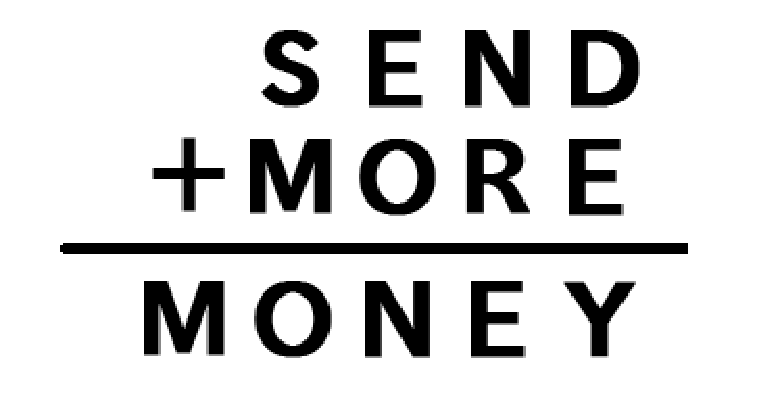
\epsfig{file=Figures/send-more-money.pdf, scale=0.4}}

\caption{A cryptarithmetic puzzle}
\label{fig:send-more-money.pdf}
\end{figure}


\noindent
A na\"ive approach to solve this problem would be to code it as a constraint satisfaction problem that has,
among others,  the
following constraint:
\\[0.2cm]
\hspace*{1.3cm}
$   (\texttt{S} \cdot 10^3 + \texttt{E} \cdot 10^2 + \texttt{N} \cdot 10 + \texttt{D}) 
  + (\texttt{M} \cdot 10^3 + \texttt{O} \cdot 10^2 + \texttt{R} \cdot 10 + \texttt{E})
  = \texttt{M} \cdot 10^4 + \texttt{O} \cdot 10^3 + \texttt{N} \cdot 10^2 + \texttt{E} \cdot 10 + \texttt{Y}
$.
\\[0.2cm]
 The problem with this constraint is that it involves far too many variables.  As this constraint can only be
 checked when all the variables have values assigned to them, the backtracking search would essentially
 boil down to a mere brute force search.  In order to do better, we have to perform the addition in Figure
 \ref{fig:send-more-money.pdf} column by column, just as it is taught in elementary school.
 \myFig{send-more-money.stlx} shows how this can be implemented in \textsc{SetlX}.

\begin{figure}[!ht]
\centering
\begin{Verbatim}[ frame         = lines, 
                  framesep      = 0.3cm, 
                  firstnumber   = 1,
                  labelposition = bottomline,
                  numbers       = left,
                  numbersep     = -0.2cm,
                  xleftmargin   = 0.0cm,
                  xrightmargin  = 0.0cm,
                ]
   createCSP := procedure() {
       Variables   := {"S", "E", "N", "D", "M", "O", "R", "Y", "C1", "C2", "C3"};
       Values      := { 0 .. 9 };
       Constraints := allDifferent({ "S", "E", "N", "D", "M", "O", "R", "Y" });
       Constraints += { '(D + E) % 10 == Y', '(D + E) \ 10 == C1',
                        '(N + R + C1) % 10 == E', '(N + R + C1) \ 10 == C2',
                        '(E + O + C2) % 10 == N', '(E + O + C2) \ 10 == C3',
                        '(S + M + C3) % 10 == O', '(S + M + C3) \ 10 == M'
                      };
       Constraints += { "S != 0", "M != 0" };
       return [Variables, Values, Constraints];
   };
\end{Verbatim}
\vspace*{-0.3cm}
\caption{Formulating ``$\texttt{SEND} + \texttt{MORE} = \texttt{MONEY}$'' as a \textsc{Csp}.}
\label{fig:send-more-money.stlx}
\end{figure}

Notice that we have introduced three additional variables ``$\texttt{C1}$'', ``$\texttt{C2}$'', ``$\texttt{C3}$''. 
These variables serve as the \href{https://en.wikipedia.org/wiki/Carry_(arithmetic)}{carry digits}.  For
example, ``$\texttt{C1}$'' is the carry digit that we get when we do the addition of the last places of the two
numbers, i.e.~we have
\\[0.2cm]
\hspace*{1.3cm}
$\texttt{D} + \texttt{E} = \texttt{C1} \cdot 10 + \texttt{Y}$.
\\[0.2cm]
This equation still contains four variables.  We can reduce it to two equations that each involve only three
variables as follows:
\\[0.2cm]
\hspace*{1.3cm}
$(\texttt{D} + \texttt{E})\; \texttt{\symbol{37}}\; 10 = \texttt{Y}$ \quad and \quad
$(\texttt{D} + \texttt{E}) \;\texttt{\symbol{92}}\; 10 = \texttt{C1}$.
\\[0.2cm]
Here, the symbol ``$\texttt{\symbol{92}}$'' denotes 
\href{https://en.wikipedia.org/wiki/Division_(mathematics)#Of_integers}{integer division}, e.g.~we have $7 \texttt{\symbol{92}} 3 = 2$.
If we try to solve the cryptarithmetic puzzle as coded in \myFig{send-more-money.stlx} using the
constraint solver developed in the previous section, we will be disappointed.  The reason is that most
constraints involve three variables and therefore the constraint propagation developed in the previous section
is of no help.  However, we can solve the problem in a few seconds if we add the following constraints for the
variables ``$\texttt{C1}$'', ``$\texttt{C2}$'', ``$\texttt{C3}$'':
\\[0.2cm]
\hspace*{1.3cm}
\texttt{"C1 < 2", "C2 < 2", "C3 < 2"}.
\\[0.2cm]
Although these constraints are certainly true, the problem with this approach is that we would prefer if our
constraint solver would be able to figure out these constraints by itself.  After all, since $\texttt{D}$ and
$\texttt{E}$ are both less than $10$, there sum is obviously less than $20$ and hence the carry $\texttt{C1}$
has to be less than $2$.  This line of reasoning is known as \blue{consistency maintenance}:
Assume that the formula $f$ is a constraint and the set of variables occurring in $f$ has the form
\\[0.2cm]
\hspace*{1.3cm}
$\texttt{Var}(f) = \{ x \} + R$ \quad where $x \not\in R$,
\\[0.2cm]
i.e.~the variable $x$ occurs in the constraint $f$ and, furthermore, $R$ is the set of all variables occurring
in $f$ that are different from $x$.  Furthermore, assume that we have a dictionary $\texttt{AllowableValues}$ such that
for every variable $y$, the dictionary entry $\texttt{AllowableValues}[y]$ is the set of values that can be substituted
for the variable $y$.  Now  \blue{a value $v$ is consistent for $x$ with respect to the constraint $f$} 
iff the partial assignment $\{ \pair(x, v) \}$ can be extended to an assignment $A$ satisfying the constraint $f$,
i.e.~for every variable $y \in R$ we have to find a value $w \in \texttt{AllowableValues}[y]$ such that the resulting
assignment $A$ satisfies the equations
\\[0.2cm]
\hspace*{1.3cm}
$\texttt{evaluate}(f, A) = \texttt{true}$.
\\[0.2cm]
Here, the function $\texttt{evaluate}$ takes a formula $f$ and an assignment $A$ and evaluates $f$ using the
assignment $A$.  Now, \blue{consistency maintenance} works as follows.
\begin{enumerate}
\item The dictionary $\texttt{AllowableValues}$ is initialized as follows:
      \\[0.2cm]
      \hspace*{1.3cm}
      $\texttt{AllowableValues}[x] := \texttt{Values}$ \quad for all $x \in \texttt{Variables}$,
      \\[0.2cm]
      i.e.~initially every variable $x$ can take any value from the set of $\texttt{Values}$.
\item Next, the set $\texttt{UncheckedVariables}$ is initialized to the set of all $\texttt{Variables}$:
      \\[0.2cm]
      \hspace*{1.3cm}
      $\texttt{UncheckedVariables} := \texttt{Variables}$.
\item As long as the set $\texttt{UncheckedVariables}$ is not empty, we remove one variable $x$ from this set:
      \\[0.2cm]
      \hspace*{1.3cm}
      $x := \texttt{from}(\texttt{UncheckedVariables})$
\item We iterate over all constraints $f$ such that $x$ occurs in $f$.  
      \begin{enumerate}
      \item For every value $v \in \texttt{AllowableValues}[x]$ we check whether $v$ is consistent with $f$.
      \item If $v$ is not consistent with $f$, then $v$ is removed from $\texttt{AllowableValues}[x]$.
            Furthermore, if $R$ is the set of all variables occurring in $f$ that are different from $x$, 
            then this set $R$ is added to the set of $\texttt{UncheckedVariables}$.
      \end{enumerate}
\item Once $\texttt{UncheckedVariables}$ is empty, the algorithm terminates.  Otherwise, we jump back to step 3
      and remove the next variable from the set $\texttt{UncheckedVariables}$.
\end{enumerate}
The algorithm terminates as every iteration removes either a variable from the set
$\texttt{UncheckedVariables}$ or it removes a value from one of the sets $\texttt{AllowableValues}[y]$ for some
variable $y$.  Although the set $\texttt{UncheckedVariables}$ can grow during the algorithm,  the union
\\[0.2cm]
\hspace*{1.3cm}
$\bigcup\limits_{x \in \mathtt{Vars}} \texttt{AllowableValues}[x]$ 
\\[0.2cm]
can never grow:  Every time the set $\texttt{UncheckedVariables}$ grows,
for some variable $x$ the set $\texttt{AllowableValues}[x]$ shrinks.
As the sets $\texttt{AllowableValues}[x]$ are finite for all variables $x$, the set
$\texttt{UncheckedVariables}$ can only grow a finite number of times. 
Once the set $\texttt{UncheckedVariables}$ does not grow any more, every iteration of the algorithm removes one
variable from this set and hence the algorithm terminates eventually.

\begin{figure}[!ht]
\centering
\begin{Verbatim}[ frame         = lines, 
                  framesep      = 0.3cm, 
                  firstnumber   = 1,
                  labelposition = bottomline,
                  numbers       = left,
                  numbersep     = -0.2cm,
                  xleftmargin   = 0.0cm,
                  xrightmargin  = 0.0cm,
                ]
    enforceConsistency := procedure(rw ValuesPerVar,
                                    Var2Formulas, Annotated, Connected)
    {
        UncheckedVars := domain(Var2Formulas);
        while (UncheckedVars != {}) {
            variable    := from(UncheckedVars);
            Constraints := Var2Formulas[variable];
            Values      := ValuesPerVar[variable];
            RemovedVals := {};
            for (f in Constraints) {
                OtherVars := Annotated[f] - { variable };
                for (value in Values) {
                    if(!existsValue(variable,value,f,OtherVars,ValuesPerVar)) {
                        RemovedVals   += { value };
                        UncheckedVars += Connected[variable];
                    }
                }
            }
            Remaining := Values - RemovedVals;
            if (Remaining == {}) { backtrack; }
            ValuesPerVar[variable] := Remaining;
        }
    };
\end{Verbatim}
\vspace*{-0.3cm}
\caption{Consistency maintenance in \textsc{SetlX}.}
\label{fig:csp-consistency.stlx:enforceConsistency}
\end{figure}

\noindent
\myFig{csp-consistency.stlx:enforceConsistency} shows how consistency maintenance can be implemented in \textsc{SetlX}.
The procedure $\texttt{enforceConsistency}$ takes four arguments.
\begin{enumerate}[(a)]
\item $\texttt{ValuesPerVar}$ is a dictionary associating the set of possible values with each variable.
\item $\texttt{Var2Formulas}$ is a dictionary.  For every variable $v$, $\texttt{Var2Formulas}[v]$ is
      the set of those constraints $f$ such that $v$ occurs in $f$.
\item $\texttt{Annotated}$ is the set of annnotated constraints, i.e. this set contains
      pairs of the form $\pair(f, V)$ where $f$ is a constraint and $V$ is the set of all variables occurring
      in $f$.  This last argument is needed only for efficiency: In order to avoid computing the set $V$ of
      variables occurring in a constraint $f$ every time the constraint $f$ is encountered, we compute these
      sets at the beginning of our computation and store them in the dictionary $\texttt{Annnotated}$.
\item $\texttt{Connected}$ is a dictionary that takes a variable $x$ and returns the set $V$ of all variables
      that are related to $x$ via a common constraint $f$, i.e.~we have $y \in \texttt{Connected}[x]$
      if there exists a constraint $f$ such that both $x$ and $y$ occur in $f$ and, furthermore, $x \not= y$.
\end{enumerate}
The procedure $\texttt{enforceConsistency}$ modifies the dictionary $\texttt{ValuesPerVar}$ so that once the
procedure has terminated, for every variable $x$ the set
$\texttt{ValuesPerVar}[x]$ is consistent with the constraints for $x$.  The implementation works as follows:
\begin{enumerate}
\item Initially, all variables need to be checked for consistency.  Therefore, $\texttt{UncheckedVars}$
      is defined to be the set of all variables that occur in any of the constraints.
\item The \texttt{while}-loop iterates as long as there are still variables $x$ left in $\texttt{UncheckedVars}$
      such that the consistency of $\texttt{ValuesPerVar}[x]$ has not been established.
\item Next, a $\texttt{variable}$ is selected and removed from $\texttt{UncheckedVars}$. 
\item $\texttt{Constraints}$ is the set of all constraints $f$ such that this $\texttt{variable}$ occurs in $f$.
\item $\texttt{Values}$ is the set of those values that can be assigned to $\texttt{variable}$.
\item $\texttt{RemovedVals}$ is the subset of those values that are found to be inconsistent with some constraint.
\item We iterate over all constraints $\texttt{f} \in \texttt{Constraints}$.
\item $\texttt{OtherVars}$ is the set of variables occurring in $\texttt{f}$ that are different from 
      the chosen $\texttt{variable}$.
\item We iterate over all $\texttt{value} \in \texttt{Values}$ that can be substituted for $\texttt{variable}$
      and check whether $\texttt{value}$ is consistent with $\texttt{f}$.   To this end, we need to find values
      that can be assigned to the variables in the set $\texttt{OtherVars}$ such that $\texttt{f}$ evaluates as
      $\texttt{true}$.  This is checked using the function $\texttt{existsValue}$.
\item If we do not find such values, then $\texttt{value}$ is inconsistent for
      $\texttt{variable}$ w.r.t.~$\texttt{f}$ and needs to be removed from the set 
      $\texttt{ValuesPerVar}[\texttt{variable}]$.  Furthermore, all variables that are connected to
      $\texttt{variables}$ have to be added to the set $\texttt{UncheckedVars}$.  The reason is that once a
      value is removed for $\texttt{variable}$, the value assigned to another variable $y$ occurring in a
      constraint that mentions both $\texttt{variable}$ and $y$ might now become inconsistent.
\item If there are no consistent values for $\texttt{variable}$ left, we have to backtrack.
\end{enumerate}

\begin{figure}[!ht]
\centering
\begin{Verbatim}[ frame         = lines, 
                  framesep      = 0.3cm, 
                  firstnumber   = 1,
                  labelposition = bottomline,
                  numbers       = left,
                  numbersep     = -0.2cm,
                  xleftmargin   = 0.8cm,
                  xrightmargin  = 0.8cm,
                  ]
    existsValue := procedure(var, val, f, Vars, ValuesPerVar) {
        AllVars := { var } + Vars;
        return exists( A in createAllAssignments(Vars, ValuesPerVar)   |
                       eval_constraint(A + { [var, val] }, f, AllVars) );
    };
    createAllAssignments := procedure(Vars, ValuesPerVar) {
        if (Vars == {}) {
            return { {} };  // set containing empty assignment
        }
        var         := from(Vars);
        Values      := ValuesPerVar[var];
        Assignments := createAllAssignments(Vars, ValuesPerVar);
        return { { [var, val] } + A : val in Values, A in Assignments };
    };
\end{Verbatim}
\vspace*{-0.3cm}
\caption{The implementation of $\texttt{existsValue}$.}
\label{fig:csp-consistency.stlx:existsValue}
\end{figure}

\noindent
\myFig{csp-consistency.stlx:existsValue} shows the implementation of the function $\texttt{existsValue}$ that
is used in the implementation of $\texttt{enforceConsistency}$.  This procedure is called with five arguments.
\begin{enumerate}[(a)]
\item $\texttt{var}$ is variable.
\item $\texttt{val}$ is a value that is to be assigned to $\texttt{var}$.
\item $\texttt{f}$ is a constraint such that $\texttt{var}$ occurs in $\texttt{f}$
\item $\texttt{Vars}$ is the set of all those other variables occurring in $\texttt{f}$, i.e.~the set of those
      variables that occur in $\texttt{f}$ but that are different from $\texttt{var}$. 
\item $\texttt{ValuesPerVar}$  is a dictionary associating the set of possible values with each variable.
\end{enumerate}
The procedure checks whether the partial assignment $\{ \pair(\texttt{var}, \texttt{val}) \}$ can be
extended so that the constraint $\texttt{f}$ is satisfied.  To this end it needs to create the set of all
possible assignments.  This set is generated using the function $\texttt{createAllAssignments}$.  This function
gets a set of variables $\texttt{Vars}$ and a dictionary that assigns to every variable $\texttt{var}$ in
$\texttt{Vars}$ the set of values that might be assigned to $\texttt{var}$.
\begin{enumerate}
\item If the set of variables $\texttt{Vars}$ is empty, the empty set can serve as a dictionary that 
      assigns a value to every variable in $\texttt{Vars}$.
\item Otherwise, we remove a variable $\texttt{var}$ from $\texttt{Vars}$ and get the set of $\texttt{Values}$
      that can be assigned to $\texttt{var}$.  
\item Recursively, we create the set of all $\texttt{Assignments}$ that associate values with the remaining 
      variables.
\item Finally, the set of all possible assignments is the set of all combinations of assigning a value 
      $\texttt{val} \in \texttt{Values}$ to $\texttt{var}$ and assigning the remaining variables according to 
      an assignment $\texttt{A} \in \texttt{Assignments}$.
\end{enumerate}
On one hand, consistency checking creates a lot of overhead.\footnote{
  To be fair, the implementation shown in this section is far from optimal.  In particular, by remembering which
  combinations of variables and values work for a given formula, the overhead can be reduced greatly.  I have
  refrained from implementing this optimization because I did not want the code to get too complex.
}
Therefore, it might actually slow down the
solution of some constraint satisfaction problems that are easy to solve using just backtracking and
propagation.  On the other hand, many difficult constraint satisfaction problems can not be solved
without consistency checking.

\section{Local Search}
There is another approach to solve constraint satisfaction problems.  This approach is known as
\blue{local search}.  The basic idea is simple: Given as constraint satisfaction problem 
$\mathcal{C}$ of the form 
\\[0.2cm]
\hspace*{1.3cm}
$\mathcal{P} := \langle \texttt{Variables}, \texttt{Values}, \texttt{Constraints} \rangle$,
\\[0.2cm] 
local search works as follows:
\begin{enumerate}
\item Initialize the values of the variables in $\texttt{Variables}$ randomly.  
\item If all $\texttt{Constraints}$ are satisfied, return the solution.
\item For every  $x \in \texttt{Variables}$, count the number of \underline{unsatisfied} constraints that involve the
      variable $x$. 
\item Set $\texttt{maxNum}$ to be the maximum of these numbers, i.e.~$\texttt{maxNum}$ is maximal number of
      unsatisfied constraints for any variable.
\item Compute the set $\texttt{maxVars}$ of those variables that have $\texttt{maxNum}$ unsatisfied constraints.
\item Randomly choose a variable $x$ from the set $\texttt{maxVars}$.
\item Find a value $d \in \texttt{Values}$ such that by assigning $d$ to the variable $x$, the number of
      unsatisfied constraints for the variable $x$ is minimized.  

      If there is more than one value $d$ with this property, choose the value $d$ randomly from those values
      that minimize the number of unsatisfied constraints.
\item Goto step 2 and repeat until either a solution is found or the sun rises in the west.
\end{enumerate}

\begin{figure}[!ht]
\centering
\begin{Verbatim}[ frame         = lines, 
                  framesep      = 0.3cm, 
                  firstnumber   = 1,
                  labelposition = bottomline,
                  numbers       = left,
                  numbersep     = -0.2cm,
                  xleftmargin   = 0.8cm,
                  xrightmargin  = 0.8cm,
                ]
    solve := procedure(n) {
        Queens := [];
        for (row in [1 .. n]) {
            Queens[row] := rnd({1 .. n});
        }
        iteration := 0;
        while (true) {
            Conflicts   := { [numConflicts(Queens, row), row] : row in [1 ..n] };
            [maxNum, _] := last(Conflicts);
            if (maxNum == 0) {
                return Queens;
            }
            if (iteration % 10 != 0) { // avoid infinite loops
                row := rnd({ row : [num, row] in Conflicts | num == maxNum });
            } else {
                row := rnd({ 1 .. n });
            }
            Conflicts := {};
            for (col in [1 .. n]) {
                Board      := Queens;
                Board[row] := col;
                Conflicts  += { [numConflicts(Board, row), col] };
            }
            [minNum, _] := first(Conflicts);
            Queens[row] := rnd({ col : [num, col] in Conflicts | num == minNum });
            iteration   += 1;
        }
    };
\end{Verbatim}
\vspace*{-0.3cm}
\caption{Solving the $n$ queens problem using local search.}
\label{fig:constraints.stlx}
\end{figure}

\noindent
\myFig{constraints.stlx} shows an implementation of these ideas in \textsc{SetlX}.  Instead of solving an
arbitrary constraint satisfaction problem, the program solves the $n$ queens problem.  We proceed to discuss
this program line by line.
\begin{enumerate}
\item The procedure $\texttt{solve}$ takes one parameter $\texttt{n}$, which is the size of the chess board.  If
      the computation is successful, $\texttt{solve(n)}$ returns a list of length $\texttt{n}$.  Lets call this
      list $\texttt{Queens}$. For every row $\texttt{r} \in \{1, \cdots, \texttt{n}\}$, the value $\texttt{Queens[r]}$ specifies that the queen 
      that resides in row $\texttt{r}$ is positioned in column $\texttt{Queens[r]}$.
\item The \texttt{for} loop initializes the positions of the queens to random values from the set
      $\{1, \cdots, \texttt{n}\}$.  Effectively, for every row on the chess board, this puts a queen in a
      random column.
\item The variable $\texttt{iteration}$ counts the number of times that we need to reassign a queen in a given row.
\item All the remaining statements are surrounded by a \texttt{while} loop that is only terminated once a
      solution has been found.
\item The variable $\texttt{Conflicts}$ is a set of pairs of the form $[c, r]$, where $c$ is the number of
      times the queen in row $r$ is attacked by other queens.  Hence, $c$ is the same as the number of
      unsatisfied conflicts for the variable specifying the column of the queen in row $r$.
\item $\texttt{maxNum}$ is the maximum of the number of conflicts for any row.
\item If this number is $0$, then all constraints are satisfied and the list $\texttt{Queens}$ is a solution to the
      $\texttt{n}$ queens problem.
\item Otherwise, we compute those rows that exhibit the maximal number of conflicts.  From these rows
      we select one $\texttt{row}$ arbitrarily.
\item The reason for enclosing the assignment to $\texttt{row}$ in an \texttt{if} statement is explained later. 
      On a first reading of  this program,  this \texttt{if} statement should be ignored.
\item Now that we have identified the $\texttt{row}$ where the number of conflicts is biggest, we need to
      reassign $\texttt{Queens[row]}$.  Of course, when reassigning this variable, we would like to have fewer
      conflicts after the reassignment.  Hence, we test all columns to find the best column that can be
      assigned for the queen in the given $\texttt{row}$.  This is done in a \texttt{for} loop that runs over
      all possible columns.  The set $\texttt{Conflicts}$ that is maintained in this loop is a set of pairs
      of the form $[k, c]$ where $k$ is the number of times the queen in $\texttt{row}$ would be attacked if it
      would be placed in column $c$.
\item We compute the minimum number of conflicts that is possible for the queen in $\texttt{row}$ and assign it
      to $\texttt{minNum}$.
\item From those columns that minimize the number of violated constraints, we choose a column randomly
      and assign it for the specified $\texttt{row}$.
\end{enumerate}
There is a technical issue, that must be addressed:  It is possible there is just one row that exhibits the
maximum number of conflicts.  It is further possible that, given the placements of the other queens, there is
just one optimal column for this row.  In this case, the procedure $\texttt{solve}$ would loop forever.  To
avoid this case, every 10 iterations we pick a random row to change.

\begin{figure}[!ht]
\centering
\begin{Verbatim}[ frame         = lines, 
                  framesep      = 0.3cm, 
                  firstnumber   = 1,
                  labelposition = bottomline,
                  numbers       = left,
                  numbersep     = -0.2cm,
                  xleftmargin   = 0.8cm,
                  xrightmargin  = 0.8cm,
                ]
    numConflicts := procedure(Queens, row) {
        n      := #Queens;
        result := 0;
        for (r in {1 .. n} | r != row) {
            if ( Queens[r] == Queens[row]           ||
                 r - Queens[r] == row - Queens[row] ||
                 r + Queens[r] == row + Queens[row]
               )
            { result += 1; }
        }
        return result;
    };
\end{Verbatim}
\vspace*{-0.3cm}
\caption{The procedure $\texttt{numConficts}$.}
\label{fig:numConficts.stlx}
\end{figure}

The procedure $\texttt{numConficts}$ shown in \myFig{numConficts.stlx} implements the function
$\texttt{numConficts}$.  Given a board $\texttt{Queens}$ that specifies the positions of the queens on the
board and a $\texttt{row}$, this function computes the number of ways that the queen in $\texttt{row}$ is
attacked by other queens.  If all queens are positioned in different rows, then there are only three ways left
that a queen can be attacked by another queen.
\begin{enumerate}
\item The queen in row $\texttt{r}$ could be positioned in the same column as the queen in $\texttt{row}$.
\item The queen in row $\texttt{r}$ could be positioned in the same falling or rising diagonal as the queen in
      $\texttt{row}$.  These diagonals are specified by the linear equations given in line 6 and 7 of Figure
      \ref{fig:numConficts.stlx}.
\end{enumerate}
Using the program discussed in this section, the n queens problem can be solved for a $\texttt{n} = 1000$ in
30 minutes.  As the memory requirements for local search are small, even much higher problem sizes can be
tackled if sufficient time is available.  Hence, it seems that local search is much better than the algorithms
discussed previously.  However, we have to note that local search is \blue{incomplete}:  If a
constraint satisfaction problem $\mathcal{P}$ has no solution, then local search loops forever.  Therefore, in
practise a dual approach is used to solve a constraint satisfaction problem.  The constraint solver starts two
threads: The first search does local search, the second thread tries to solve the problem via some refinement
of backtracking.  the first thread that terminates wins.  The resulting algorithm is complete and, for a
solvable problem, will have similar performance as local search.  If the problem is unsolvable, this will
\blue{eventually} be discovered by backtracking.  Note, however, that the constraint satisfaction
problem is NP-complete.  Hence, it is unlikely that there is an efficient algorithm that works always.
However, many practically occurring constraint satisfaction problems can be solved today in a reasonably short
time. 

%%% Local Variables:
%%% mode: latex
%%% TeX-master: "artificial-intelligence"
%%% End:
